\setcounter{chapter}{23}
\chapter{Anhang}
\pagenumbering{Roman}

% \section{Basis Kapillarrheometer}
% Quelle: GÖTTFERT Werkstoff-Prüfmaschinen GmbH
% \begin{figure}[ht]
%     \begin{center}
%         \includegraphics[width=0.75\textwidth]{assets/img/DE_IMG_Prinzip_Kapillarrheometer.png}
%         \caption{Basis Kapillarrheometer}
%         \label{base_capillary_rheometer}
%     \end{center}
% \end{figure}
% \clearpage



% % \section{Detaillierte Zeitplanung nach Phasen}
% \begin{table}[ht]
%     \begin{center}
%         \begin{tabular}{| l | r  r |}
%             \hline
%             \textbf{Projektphase}                                & \multicolumn{2}{ c |}{\textbf{Zeit in h}}                \\
%             \hline

%             \textbf{Planungsphase}                               &                                           & \textbf{80} \\
%             \hline
%             \tabindent{IST-Analyse}                              & 20                                        &              \\
%             \hline
%             \tabindent{SOLL-Konzept}                             & 20                                        &              \\
%             \hline
%             \tabindent{Ablaufplanung}                            & 20                                        &              \\
%             \hline
%             \tabindent{Zeit- und Ressourcenplanung}              & 20                                        &              \\
%             \hline

%             \textbf{Durchführung}                                &                                           & \textbf{280} \\
%             \hline
%             \tabindent{Automation Mess- und Kalibrierprozess}    &                                           & 160          \\
%             \hline
%             \doubletabindent{Ablauf Temperaturmessung}           & 80                                       &              \\
%             \hline
%             \doubletabindent{Datenspeicherung}                   & 80                                        &              \\
%             \hline
%             \tabindent{Datentransfer und Auswertung}             &                                           & 120          \\
%             \hline
%             \doubletabindent{Datentransfer}                      & 40                                        &              \\
%             \hline
%             \doubletabindent{Integration PowerTool}              & 40                                        &              \\
%             \hline
%             \doubletabindent{Ermittlung Korrekturwert}           & 20                                        &              \\
%             \hline
%             \doubletabindent{Erstellung Prozessprotokoll}        & 20                                        &              \\
%             \hline

%             \textbf{Testphase/Abnahme}                           &                                           & \textbf{40}  \\
%             \hline
%             \tabindent{Testen einzelner Komponenten}             & 16                                        &              \\
%             \hline
%             \tabindent{Testen im Livebetrieb}                    & 16                                         &              \\
%             \hline
%             \tabindent{Abnahme durch Projektteam}                & 8                                        &              \\
%             \hline

%             \textbf{Auswertung/Fazit/Dokumentation}              &                                           & \textbf{80} \\
%             \hline
%             \tabindent{Auswertung: Gewinn durch Automatisierung} & 8                                        &              \\
%             \hline
%             \tabindent{Projekt-Dokumentation}                    & 72                                        &              \\

%             \hline \hline
%             \textbf{Gesamt}                                      &                                           & \textbf{480} \\
%             \hline
%         \end{tabular}
%     \end{center}
%     \caption{Detaillierte Zeitplanung nach Phasen}
%     \label{zeitplanung-detail}
% \end{table}
% \clearpage

\section{Arduino Uno R3 Datasheet}\label{arduino_datasheet}
\cite[Arduino, Webseite abgerufen am 20.12.2022]{arduino_datasheet}
% Quelle: GÖTTFERT Werkstoff-Prüfmaschinen GmbH
%  \begin{figure}[ht]
%     \begin{center}
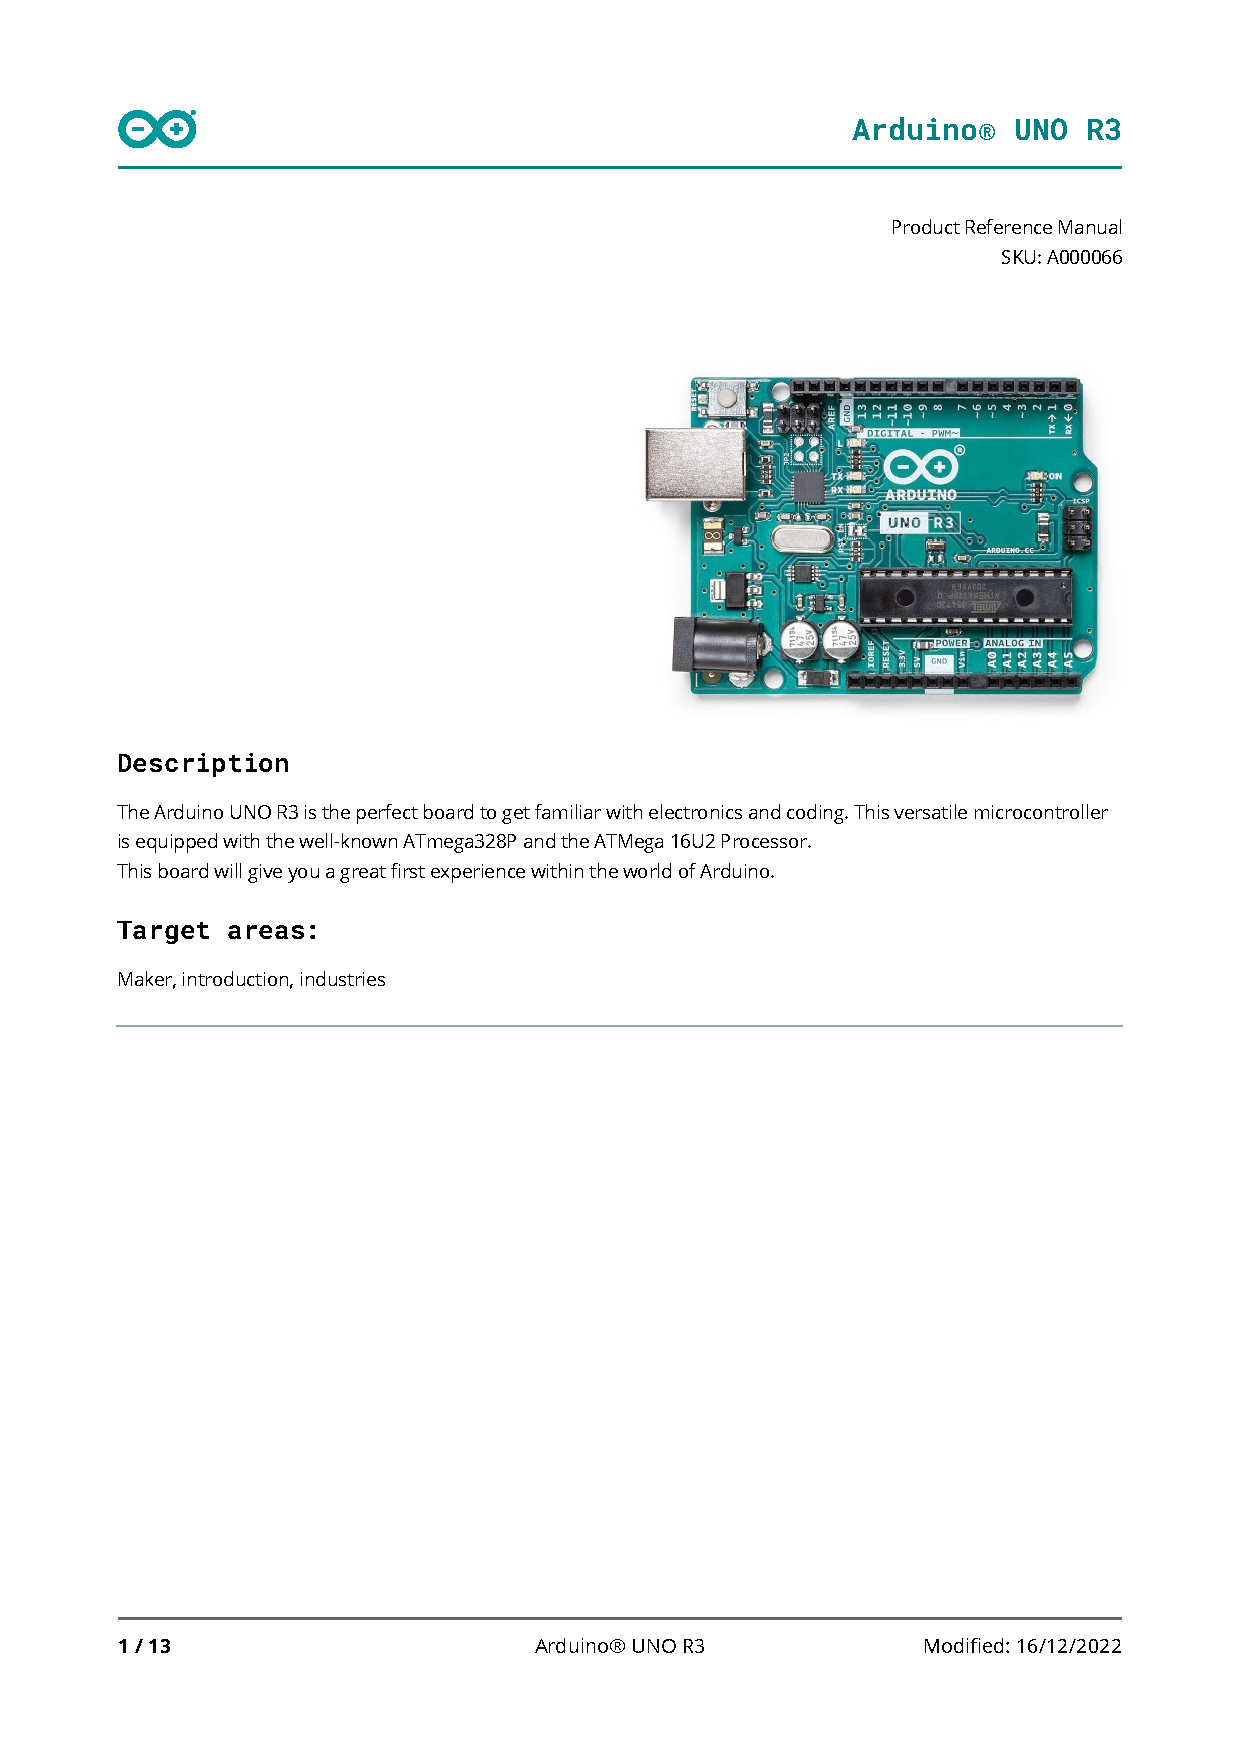
\includepdf[pages=-, landscape=true]{assets/doc/A000066-datasheet.pdf}

% %  \includegraphics[width=1.4\textwidth, angle=90]{assets/pdf/012.06.0.04.628.0_DOKU.pdf}
% %  \caption{Zeichnung Heißkanal RHEOGRAPH}

% %     \end{center}
% %  \end{figure}
% \clearpage
